\section{Method}
\label{sec:Method}
%This section describes the steps taken in this project. First the collection and the annotation of the dataset is explained. Thereafter the used algorithms are described in detail. The code used in this project can be found in appendix \ref{sec:ap-code}
This section describes the steps undertaken in this project.
First the pipeline is explained, after which the details of the implementation are stated.

\subsection{Pipeline}
\label{sec:Method-pipeline}
As stated in section \ref{sec:Theory}, a CNN was used as a feature-vector of the image, after which a Support Vector Machine was used for classification.

Several libraries exist that implement a CNN.
In this project, the choice was made to use Caffe \citep{jia2014caffe} because this framework is open source and free to use.
Moreover, it has a large community maintaining and developing, can run both on CPU and GPU and has an interface to \texttt{Python}.

The Caffe framework has several pre-trained CNNs.
In this project the Caffenet network was used, which is an implementation of Alexnet \citep{krizhevsky2012imagenet}. Caffenet is trained on the \textit{ilsvrc12} dataset, however in contrary to Alexnet, the order of pooling and normalisation is swapped.

The output of Caffenet is a $1\times1.000$ probability vector, representing the confidence of the respective class.
However, the second-to-last layer of the network is used as feature-vector. This layer is a $10\times4.096$ vector; $10$ rows because the network uses five overlapping `sub-images' (four corners and one centre) and their mirrored image, to improve accuracy.
Each row of $4.096$ numbers is an abstract representation of the image, trained by the network.
To reduce complexity, the mean over the `sub-images' is used to compress the second-to-last layer data in a $1\times4.096$ vector.
This vector was then used as a $4.096$ dimensional space for the SVM.
The three possible hyperplanes as described in section \ref{sec:Theory-class} were tested using several parameters.
Tests were conducted by training the SVM on the test-data, and using the validate-data to find the best parameters.
Figure \ref{fig:pipeline} shows a visualisation of the pipeline used in this project.

Three different types of hyperplanes were used.
A polygonal plane was tested with degrees of $2$ till $9$.
An RBF plane was tested with gammas of $0.0$ till $1.0$ with steps of $0.1$.
Lastly a linear plane was tested.
Each of the twenty SVM models were trained on part of the train-set, with intervals of order of magnitude; the sizes of the train-set were: 14, 140, 1.400 and 14.000 images.

\begin{figure}
\centering
\ifx\showfig\undefined
\centerline{
\begin{minipage}{\widefigwidth}
\tikzstyle{image} = [rectangle, draw, fill=blue!20, 
    text width=1.5cm, text centered, minimum height=1cm]
\tikzstyle{cnn} = [rectangle, draw, fill=orange!40,
    text width=2cm, text centered, rounded corners, minimum height=1cm]
\tikzstyle{vector10} = [rectangle, draw, fill=gray!40, 
    text width=1.5cm, text centered, rounded corners, minimum height=1cm]
\tikzstyle{vector1} = [rectangle, draw, fill=gray!20, 
    text width=1.5cm, text centered, rounded corners, minimum height=1cm]
\tikzstyle{svm} = [rectangle, draw, fill=purple!20, 
    text width=1.5cm, text centered, rounded corners, minimum height=1cm]
\tikzstyle{output} = [rectangle, fill=white!0,
    text width=4cm, text centered, rounded corners, minimum height=1cm]
\tikzstyle{labm} = [rectangle, text width=2cm, 
	text centered, minimum height=1cm]
\tikzstyle{line} = [draw, -latex']
\resizebox{\textwidth}{!}{
\begin{tikzpicture}[node distance = 0.5cm, auto]
	\node [image] (a) at (-7,0) {Image};
	\node [labm, above= of a] (at) {Input};
%
	\node [cnn, right=of a] (b) {Caffenet};
	\node [labm, above= of b] (bt) {CNN};
%
	\node [vector10, right=of b] (c) {$10\times4096$};
	\node [labm, above= of c] (ct) {Feature-vector};
%
	\node [vector1, right= of c] (d) {$1\times4096$};
	\node [labm, above= of d] (dt) {Feature-vector};
%
	\node [svm, right= of d] (e) {Animals};
	\node [svm, below= of e] (f) {Plastic};
	\node [labm, above= of e] (et) {SMV};
%
	\node [output, right= of e] (g) {$[0,1]$ showing animals};
	\node [output, right= of f] (h) {$[0,1]$ showing plastic};
	\node [labm, above= of g] (gt) {Output};
%
%
	\path [line] (a) -- (b);
	\path [line] (b) -- (c);
	\path [line] (c) -- (d);
	\path [line] (d) -- (e);
	\path [line] (d) -- (f);
	\path [line] (e) -- (g);
	\path [line] (f) -- (h);
\end{tikzpicture}
}
\end{minipage}
} \fi
\caption{Schematics of pipeline used in this project. The image is classified using a CNN, the mean of the second-to-last layer is input for two SVMs which give the output whether detecting plastic or animals.}
\label{fig:pipeline}
\end{figure}


\subsection{Implementation}
\label{sec:Method-implementation}
{\Python} was used to write the code necessary for the pipeline.
This choice was made not only because Caffe has an interface in \Python, but also because of the many libraries available in \Python.
The library that allows the use of matrices and basic linear algebra operations is \texttt{numpy}.
Another library called \texttt{scikit.learn} has an implementation of an SVM, which has been used in this project.

All models were trained and tested on a laptop with 2$^{nd}$ generation i5 CPU, 4GB RAM and without using a GPU. Therefore, the testing and training time of this project should be evaluated relatively to each other.
Furthermore, because no GPU was used, running Caffenet took a considerable amount of time. Therefore the output of the network was saved for each image, in order to speed up the training of the SVM.

\subsection{Detecting the location of plastic}
\label{sec:Method-location}
After testing the pipeline to detect plastic and marine life on images, small adaptations were made in order to find the location of the classes in the images.
When the system developed in this project is eventually used for practical applications, finding the exact location of the plastic will be important.

To distinguish blobs in an image, several techniques could be used; however, as a prove of feasibility, no complex algorithms were used in this project.
A new piece of code was written that segmented the image in sections and treated each of them as an image in the original pipeline.

The outcome of each segmented piece of the image was cumulated to show the confidence of detection of the classes at the given location in the image.
Because there was no labelled data of these segmented images, the evaluation could not be done on a large scale.
Therefore no sizeable experiments could be conducted to test the accuracy of locating of the classes.
However, in section \ref{sec:Results-location} the outcome of several tests is shown.

\begin{figure}%[h!tb]
\centering
\ifx\showfig\undefined
\tikzstyle{image} = [rectangle, draw, fill=blue!20, 
    text width=1.5cm, text centered, minimum height=1cm]
\tikzstyle{imaged} = [rectangle, draw, fill=blue!20, 
    text width=.74cm, text centered, minimum height=.45cm]
\tikzstyle{imagedd} = [rectangle, draw, fill=blue!20, 
    text width=.3cm, text centered, minimum height=.15cm]
%
\tikzstyle{orpi} = [rectangle, draw, fill=orange!40,
    text width=2cm, text centered, rounded corners, minimum height=1cm]
%
\tikzstyle{pimage} = [rectangle, draw, fill=red!20, 
    text width=1.5cm, text centered, minimum height=1cm]
\tikzstyle{pimaged} = [rectangle, draw, fill=red!20, 
    text width=.74cm, text centered, minimum height=.45cm]
\tikzstyle{pimagedd} = [rectangle, draw, fill=red!20, 
    text width=.3cm, text centered, minimum height=.15cm]
%
\tikzstyle{aimage} = [rectangle, draw, fill=green!20, 
    text width=1.5cm, text centered, minimum height=1cm]
\tikzstyle{aimaged} = [rectangle, draw, fill=green!20, 
    text width=.74cm, text centered, minimum height=.45cm]
\tikzstyle{aimagedd} = [rectangle, draw, fill=green!20, 
    text width=.3cm, text centered, minimum height=.15cm]
%
\tikzstyle{cnn} = [rectangle, draw, fill=orange!40,
    text width=2cm, text centered, rounded corners, minimum height=1cm]
\tikzstyle{vector10} = [rectangle, draw, fill=gray!40, 
    text width=1.5cm, text centered, rounded corners, minimum height=1cm]
\tikzstyle{vector1} = [rectangle, draw, fill=gray!20, 
    text width=1.5cm, text centered, rounded corners, minimum height=1cm]
\tikzstyle{svm} = [rectangle, draw, fill=purple!20, 
    text width=1.5cm, text centered, rounded corners, minimum height=1cm]
\tikzstyle{output} = [rectangle, fill=white!0,
    text width=4cm, text centered, rounded corners, minimum height=1cm]
\tikzstyle{labm} = [rectangle, text width=2cm, 
	text centered, minimum height=1cm]
\tikzstyle{line} = [draw, -latex']
\def\elwi{2cm}
\def\I{
\resizebox{\elwi}{!}{
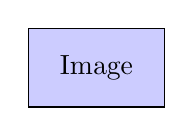
\begin{tikzpicture}
	\node [image] (a) at (0,0) {Image};
\end{tikzpicture}
} }
\def\Id{
\resizebox{\elwi}{!}{
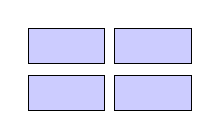
\begin{tikzpicture}
	\node [imaged] (ba) at (-4,.3) {};
	\node [imaged] (bb) at (-2.9,-.3) {};
	\node [imaged] (bc) at (-4,-.3) {};
	\node [imaged] (bd) at (-2.9,.3) {};
\end{tikzpicture}
} }
\def\Idd{
\resizebox{\elwi}{!}{
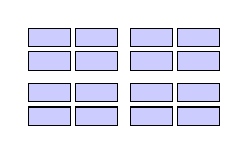
\begin{tikzpicture}
	\node [imagedd] (caa) at (2.3,.5) {};
	\node [imagedd] (cab) at (2.3,.2) {};
	\node [imagedd] (cac) at (1.7,.5) {};
	\node [imagedd] (cad) at (1.7,.2) {};
	%
	\node [imagedd] (cba) at (3,.5) {};
	\node [imagedd] (cbd) at (3,.2) {};
	\node [imagedd] (cbc) at (3.6,.5) {};
	\node [imagedd] (cbd) at (3.6,.2) {};
	%
	\node [imagedd] (cca) at (2.3,-.5) {};
	\node [imagedd] (ccb) at (2.3,-.2) {};
	\node [imagedd] (ccc) at (1.7,-.5) {};
	\node [imagedd] (ccd) at (1.7,-.2) {};
	%
	\node [imagedd] (cda) at (3,-.5) {};
	\node [imagedd] (cdb) at (3,-.2) {};
	\node [imagedd] (cdc) at (3.6,-.5) {};
	\node [imagedd] (cdd) at (3.6,-.2) {};
\end{tikzpicture}
} }
\def\ori{
\resizebox{\elwi}{!}{
\begin{tikzpicture}
	\node [orpi] (p) at (0.0) {Original\\pipeline};
\end{tikzpicture}
} }
\def\red{
\resizebox{\elwi}{!}{
\begin{tikzpicture}
	\node [pimage] (p) at (0.0) {Plastic};
\end{tikzpicture}
} }
\def\Rd{
\resizebox{\elwi}{!}{
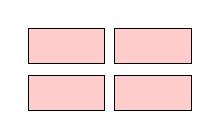
\begin{tikzpicture}
	\node [pimaged] (ba) at (-4,.3) {};
	\node [pimaged] (bb) at (-2.9,-.3) {};
	\node [pimaged] (bc) at (-4,-.3) {};
	\node [pimaged] (bd) at (-2.9,.3) {};
\end{tikzpicture}
} }
\def\Rdd{
\resizebox{\elwi}{!}{
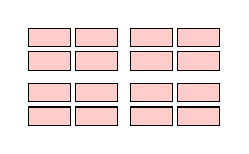
\begin{tikzpicture}
	\node [pimagedd] (caa) at (2.3,.5) {};
	\node [pimagedd] (cab) at (2.3,.2) {};
	\node [pimagedd] (cac) at (1.7,.5) {};
	\node [pimagedd] (cad) at (1.7,.2) {};
	%
	\node [pimagedd] (cba) at (3,.5) {};
	\node [pimagedd] (cbd) at (3,.2) {};
	\node [pimagedd] (cbc) at (3.6,.5) {};
	\node [pimagedd] (cbd) at (3.6,.2) {};
	%
	\node [pimagedd] (cca) at (2.3,-.5) {};
	\node [pimagedd] (ccb) at (2.3,-.2) {};
	\node [pimagedd] (ccc) at (1.7,-.5) {};
	\node [pimagedd] (ccd) at (1.7,-.2) {};
	%
	\node [pimagedd] (cda) at (3,-.5) {};
	\node [pimagedd] (cdb) at (3,-.2) {};
	\node [pimagedd] (cdc) at (3.6,-.5) {};
	\node [pimagedd] (cdd) at (3.6,-.2) {};
\end{tikzpicture}
} }
\def\gre{
\resizebox{\elwi}{!}{
\begin{tikzpicture}
	\node [aimage] (p) at (0.0) {Animals};
\end{tikzpicture}
} }
\def\Gd{
\resizebox{\elwi}{!}{
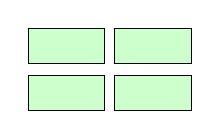
\begin{tikzpicture}
	\node [aimaged] (b1) at (-4,.3) {};
	\node [aimaged] (b2) at (-2.9,-.3) {};
	\node [aimaged] (b3) at (-4,-.3) {};
	\node [aimaged] (b4) at (-2.9,.3) {};
\end{tikzpicture}
} }
\def\Gdd{
\resizebox{\elwi}{!}{
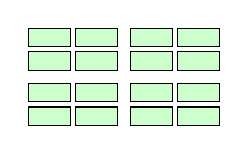
\begin{tikzpicture}
	\node [aimagedd] (caa) at (2.3,.5) {};
	\node [aimagedd] (cab) at (2.3,.2) {};
	\node [aimagedd] (cac) at (1.7,.5) {};
	\node [aimagedd] (cad) at (1.7,.2) {};
	%
	\node [aimagedd] (cba) at (3,.5) {};
	\node [aimagedd] (cbd) at (3,.2) {};
	\node [aimagedd] (cbc) at (3.6,.5) {};
	\node [aimagedd] (cbd) at (3.6,.2) {};
	%
	\node [aimagedd] (cca) at (2.3,-.5) {};
	\node [aimagedd] (ccb) at (2.3,-.2) {};
	\node [aimagedd] (ccc) at (1.7,-.5) {};
	\node [aimagedd] (ccd) at (1.7,-.2) {};
	%
	\node [aimagedd] (cda) at (3,-.5) {};
	\node [aimagedd] (cdb) at (3,-.2) {};
	\node [aimagedd] (cdc) at (3.6,-.5) {};
	\node [aimagedd] (cdd) at (3.6,-.2) {};
\end{tikzpicture}
} }
\def\Pla{
\resizebox{\elwi}{!}{
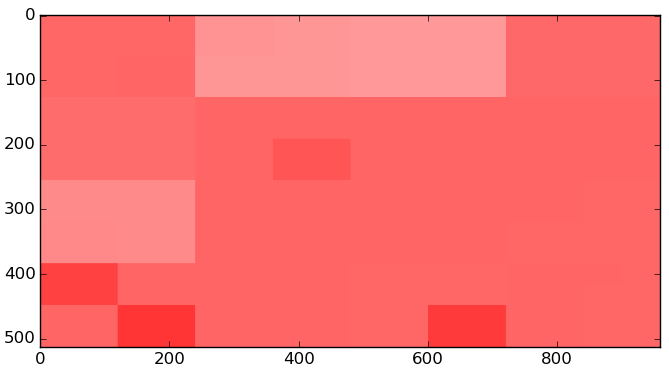
\includegraphics{images/segment/253_01__plastic__.png}
%\begin{tikzpicture}
%	\node [orpi] (p) at (0.0) {Original\\Pipeline};
%\end{tikzpicture}
} }
\def\Ani{
\resizebox{\elwi}{!}{
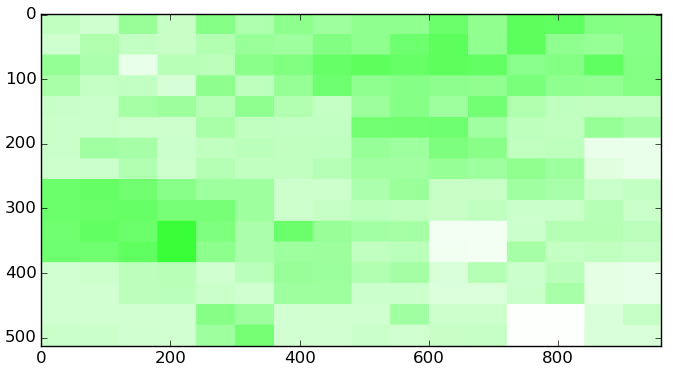
\includegraphics{images/segment/253_01__animals__.png}
%\begin{tikzpicture}
%	\node [orpi] (p) at (0.0) {Original\\Pipeline};
%\end{tikzpicture}
} }
\def\mdo{
\resizebox{\elwi}{!}{
\begin{tikzpicture}
	\node [labm] (p) at (0.0) {...};
\end{tikzpicture}
} }
\centerline{
\begin{minipage}{\widefigwidth}
\resizebox{\textwidth}{!}{
\xymatrix{
\I \ar[r]^{devide} \ar[d]^{\times2^0}& \Id \ar[r]^{devide} \ar[d]^{\times2^1}& ... \ar[r]^{devide} \ar[d]& \Idd \ar[d]^{\times2^d}& \\
\ori \ar[d]& \ori \ar[d]& \mdo \ar[d]& \ori \ar[d]& \\
\red \ar[r]^{+}& \Rd \ar[r]^{+}& \mdo \ar[r]^{+}& \Rdd \ar[r]^{=}& \Pla\\
\gre \ar[r]^{+}& \Gd \ar[r]^{+}& \mdo \ar[r]^{+}& \Gdd \ar[r]^{=}& \Ani\\
}
}
\end{minipage}
}

\fi
\caption{Schematics of the second pipeline for localisation. The image is segmented into pieces. Each piece is pulled through the original pipeline, resulting in images with intensity according to the output of the SVM. All the pieces are added together at the pixel-location, which results in an image showing the confidence of the location of plastic or animals}
\label{fig:locpip}
\end{figure}









\iffalse
\subsection{Algorithm}
\label{sec:Method-algotihm}
\todo{structuur: -ding, -implementatie}
Because of the high accuracy Convolutional Neural Networks (CNNs) have reached on several problems in Computer Vision, they are also used in this project.
As stated in section \ref{sec:Method-Data}, this project will not train a CNN, but make use of a pre-trained one.
This not only because of the high chance of over-fitting on the data, but also because a pre-trained CNN has already learned basic visual concepts.
The first layers of a CNN consist of abstract representations of lines, corners and other gradients \citep{zeiler2014visualizing}.
Unnecessarily training a network on these concepts would be a waste of time.

Moreover floating plastic and animals, the classes that are trained in this project, consist of several distinctive features that are probably learnt by the network in higher layers of abstraction.
The second-to-last layer of the network consist of an abstract representation of the image.
This layer will probably have the information needed to classify the images. \citeneed

The output of this second-to-last layer will then be used to train several algorithms to research which will perform best.
The different algorithms are stated in detail below and the results of each algorithm can be found in tion}
After testing the pipeline to detect plastic and marine life on images, small adaptations were made tosection \ref{sec:Results} \todo{deze alinea uitbreiden}
\todo{pipeline en evaluatie }

\subsubsection{Convolutional Neural Network}
\label{sec:Method-CNN}
\todo{dit een stuk korter/vlotter/to-the-point (motivatie in theory)}
%How the algorithm from section CNN is used here... caffe framework (and why)...
In section \ref{sec:Theory-CNN} and \ref{sec:Method-Algorithm} the usage of Convolutional Neural Networks (CNNs) is funded.
In this section the chosen framework and network will be explained in detail.

Several libraries exist that implement a CNN.
In this project the choice is made to use Caffe \citep{jia2014caffe}.
This framework is open source and free to use.
Moreover it has a large community maintaining and developing, can run both on CPU and GPU and has an interface to \texttt{Python}.

The Caffe framework has several pre-trained CNNs.%, including GoogleNet.
However, to reduce computation needed, a smaller network called Caffenet.
This is an implementation of Alexnet \citet{krizhevsky2012imagenet} with small diferences, trained on the \textit{ilsvrc12} dataset. \citeneed
This network segments the image in five overlapping `sub-images' (four corners and one centre) and their mirrored image, to improve accuracy.

Every image in the dataset has been pulled through the network, after which the data of the last and second-to-last layer has been saved.
The data of the last layer of the network is returned as a \texttt{numpy}\footnote{\texttt{numpy} is a \texttt{Python} library used for linear algebra} array of size $1\times1.000$.
The numbers in this array represent the probability the given image belongs to the respective class.
The second-to-last layer, called \textit{fc7} in this network, is a \texttt{numpy} array of size $10\times4.096$.
The $4.096$ columns are the abstract representation of the image, where the $10$ rows represent the different `sub-images'.
The data was stored on a hard-drive to speed-up further calculations.

%\subsubsection{Principal Component Analysis}
%\label{sec:Method-PCA}
%\todo{rede verzinnen waarom dit gedaan is}

\subsubsection{Feed Forward Network}
\label{sec:Method-FFN}
\todo{dit stuk weg}
To classify the second-to-last layer in the two classes of this project, a Feed Forward Neural Network (FFN) has been used.
This network has a structure of three layers: the input layer, the hidden layer and the output layer.
The implementation of this network has not been made in this project, but a \texttt{Python} implementation of \citeneed is used.
The input layer of $4.096$ nodes, one for each output of the CNN, and output layer of two nodes, one for each of the classes, were immutable.
Different numbers of nodes in the hidden layer were tested, even so the normalisation of the data.

The train-set has been used for training, and the validate-set has been used to distinguish between the different parameters.

The output of this network, shown in section \ref{sec:Results-FFN}, was not satisfactory, therefore the use of SVMs was researched further.

\subsubsection{Support Vector Machine}
\label{sec:Method-SVM}
After testing the FFN, the choice was made to use a Support Vector Machine (SVM).
In this case the implementation of \texttt{scikit.learn} of SVMs is used.
The second-to-last layer output constructs a $4.096$ dimensional space were the data represents points.
To speed up computation the mean of the `sub-images' is used to reduce the number of data-points.

The same method as with FFN regarding fitting the data and parameters on the train- and validate-set was used.
The results are shown in section \ref{sec:Results-SVM}.

\subsubsection{Detecting location of plastic}
\label{sec:Method-sub}
After several tests with a SVM, locating plastic within the image was researched.
Several techniques could be used to distinguish blobs, however, as a prove of feasibility, no complex algorithms were used.
A new piece of code was written that segments the image in sections and treats each of them as an image in the original pipeline.

Because there is not labelled data of these segmented images, the evaluation could not be done on a large scale.
Therefore no sizable experiments could be conducted to test the accuracy of locating of the classes.
However, in section \ref{sec:Results-sub} the outcome of several test is shown.

\fi